\documentclass[tikz]{standalone}

\usetikzlibrary{matrix}
\usetikzlibrary{positioning}
\usetikzlibrary{patterns}
\usetikzlibrary{decorations.markings}
\usetikzlibrary{arrows}
\usetikzlibrary{arrows.meta}
\usetikzlibrary{backgrounds}
\usetikzlibrary{math}

\definecolor{textColor}{RGB}{248, 248, 255}
\definecolor{bgColor}{rgb}{0.3, 0.3, 0.3}

\begin{document}
    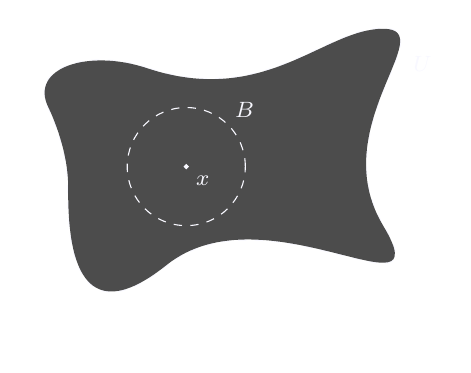
\begin{tikzpicture}
        \newcommand{\pathA}{(-0.50,+1.25) .. controls (+1.00,+0.75) and (+1.75,+1.75) .. (+2.50,+1.75)}
        \newcommand{\pathB}{(+2.50,+1.75) .. controls (+3.25,+1.75) and (+1.75,+0.50) .. (+2.50,-0.75)}
        \newcommand{\pathC}{(+2.50,-0.75) .. controls (+3.25,-2.00) and (+1.00,-0.25) .. (-0.25,-1.25)}
        \newcommand{\pathD}{(-0.25,-1.25) .. controls (-1.50,-2.25) and (-1.50,-0.75) .. (-1.50,-0.25)}
        \newcommand{\pathE}{(-1.50,-0.25) .. controls (-1.50,+0.25) and (-1.75,+0.75) .. (-1.75,+0.75)}
        \newcommand{\pathF}{(-1.75,+0.75) .. controls (-2.00,+1.25) and (-1.25,+1.50) .. (-0.50,+1.25)}
        \draw[dashed, thick, dash phase=11pt, color=textColor] \pathA -- \pathB -- \pathC -- \pathD -- \pathE -- \pathF -- cycle;
        \fill[color=bgColor] \pathA -- \pathB -- \pathC -- \pathD -- \pathE -- \pathF;
        \draw (3,1.3) circle (0) node[text=textColor] {\footnotesize{$U$}};
        \filldraw[color=textColor] (0,0) circle (0.25mm) node[below right, text=textColor] {\footnotesize{$x$}};
        \draw[dashed, color=textColor] (0,0) circle (0.75) node[above right=7mm, text=textColor] {\footnotesize{$B$}};
    \end{tikzpicture}
\end{document}
